% Setting up document class and basic structure
\documentclass[11pt]{article}

% Including essential packages for formatting and content
\usepackage[a4paper, margin=1in]{geometry}
\usepackage{amsmath, amssymb}
\usepackage{graphicx}
\usepackage{hyperref}
\usepackage{enumitem}
\usepackage{titlesec}
\usepackage{xcolor}
\usepackage{parskip}
\usepackage{booktabs}
\usepackage{caption}

% Configuring hyperlinks
\hypersetup{
    colorlinks=true,
    linkcolor=blue,
    urlcolor=blue,
    citecolor=blue
}

% Setting up fonts (using standard PDFLaTeX fonts)
\usepackage[T1]{fontenc}
\usepackage{lmodern}

% Customizing section titles
\titleformat{\section}{\large\bfseries}{\thesection}{1em}{}
\titleformat{\subsection}{\normalsize\bfseries}{\thesubsection}{1em}{}

% Defining custom colors
\definecolor{headerblue}{RGB}{0, 51, 102}

% Starting the document
\begin{document}

% Creating the title section
\begin{center}
    {\Huge \textbf{MotorDrive: Open-Source BLDC Motor Driver}}\\
    \vspace{0.2cm}
    {\large \textit{Design: Motor Driver with Bluetooth}}\\
    \vspace{0.1cm}
    {\normalsize Engineer: Cy Drollinger \quad | \quad Date: June 2025 \quad | \quad Email: \href{mailto:cydrollinger@gmail.com}{cydrollinger@gmail.com}}
\end{center}

\vspace{0.5cm}

% Including the main image
\begin{figure}[h]
    \centering
    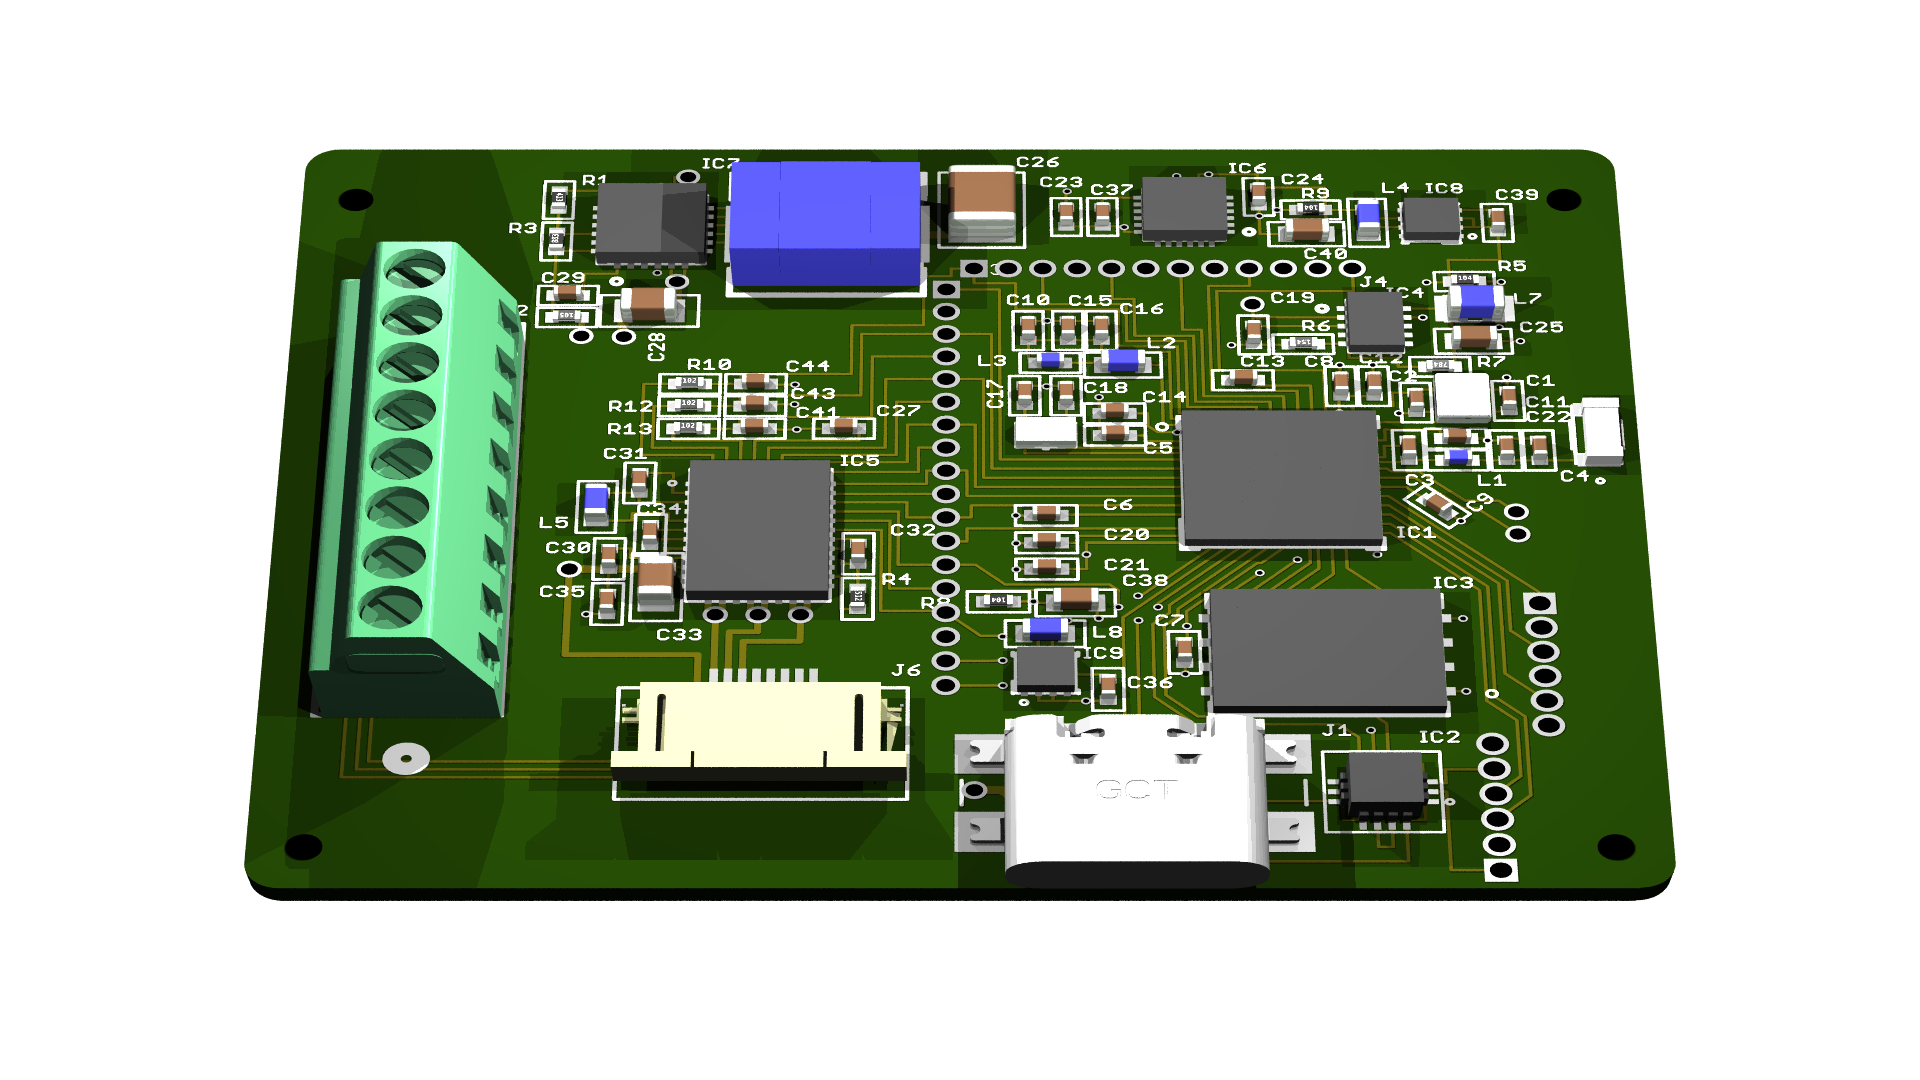
\includegraphics[width=0.6\textwidth]{motorDRVjlc.png}
    \caption{MotorDrive Prototype Design}
    \label{fig:motorDRV}
\end{figure}

% Purpose section
\section{Purpose}
The MotorDrive project aims to develop an open-source, cost-effective three-phase brushless DC (BLDC) motor driver with Bluetooth connectivity. Our goal is to build a global team of contributors to create a turn-key hardware solution for applications in robotics, electric vehicles, drones, and IoT devices. The prototype is designed for seamless manufacturing at \href{https://jlcpcb.com}{JLCPCB}, enabling anyone to produce a high-quality BLDC driver at minimal cost.

% Project Overview section
\section{Project Overview}
MotorDrive is a fully open-source BLDC motor driver featuring:
\begin{itemize}[leftmargin=*]
    \item \textbf{Hardware}: A 6-layer PCB optimized for low-cost production at JLCPCB.
    \item \textbf{Bluetooth}: Wireless control and real-time data monitoring.
    \item \textbf{Applications}: Suitable for robotics, EVs, drones, and industrial automation.
    \item \textbf{Firmware}: Planned integration with Zephyr RTOS for robust embedded control.
\end{itemize}
The repository provides all necessary files for manufacturing, including Gerber files, bill of materials (BOM), and component placement lists, making it easy to replicate the prototype.

% Manufacturing Instructions section
\section{Manufacturing Instructions}
To produce the MotorDrive prototype at \href{https://jlcpcb.com}{JLCPCB}, upload the following files:
\begin{enumerate}
    \item \texttt{gerber/jlcpcb6lyr.zip}: Gerber files for the 6-layer PCB.
    \item \texttt{manufacturing/DRVjlc(2)\_top\_cpl.csv}: Component placement list.
    \item \texttt{manufacturing/DRVjlc(2)\_top\_bom.csv}: Bill of materials.
\end{enumerate}
These files enable turn-key manufacturing, resulting in the following hardware model:

\begin{figure}[h]
    \centering
    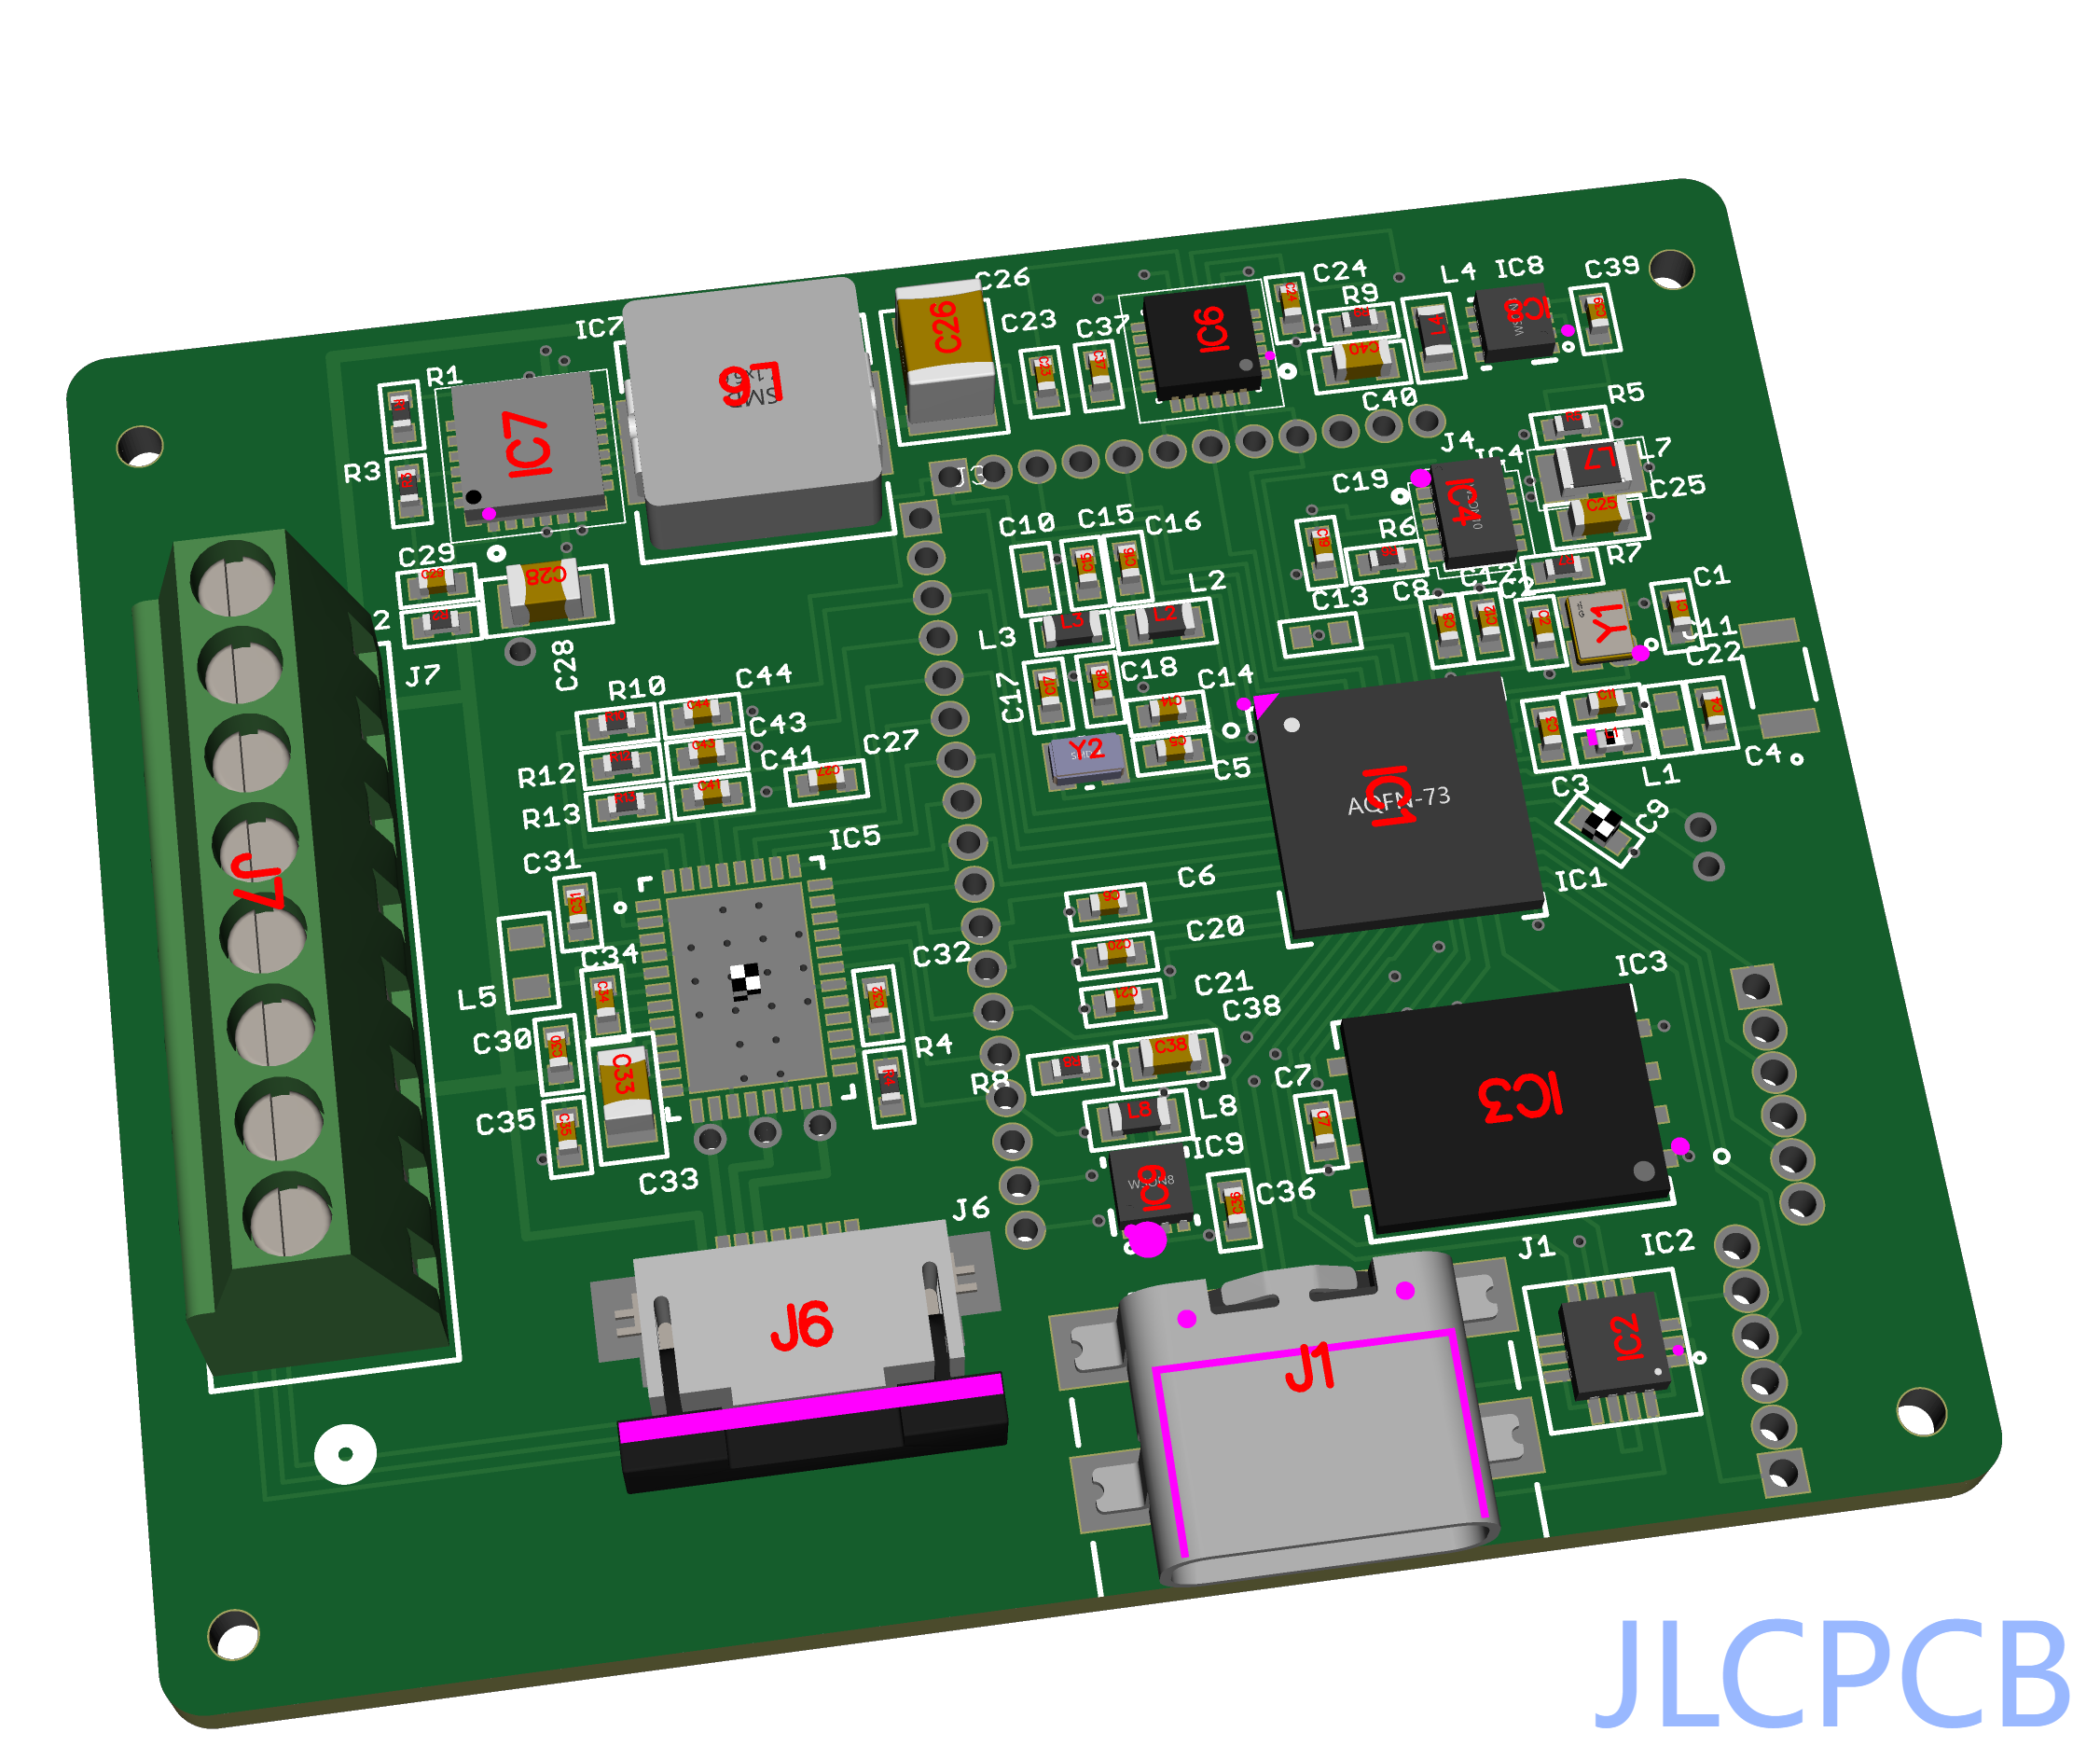
\includegraphics[width=0.6\textwidth]{jlcII.png}
    \caption{MotorDrive Hardware Model (JLCPCB)}
    \label{fig:jlcII}
\end{figure}

% Setup and Testing section
\section{Setup and Testing}
To get started with the MotorDrive prototype:
\begin{enumerate}
    \item \textbf{Manufacture the PCB}: Follow the manufacturing instructions above to order from JLCPCB.
    \item \textbf{Assemble Components}: Ensure all components listed in the BOM are correctly placed.
    \item \textbf{Flash Firmware}: Clone the repository and follow the firmware setup guide (coming soon) to program the driver.
    \item \textbf{Test the Driver}: Connect a BLDC motor and use a Bluetooth-enabled device to test basic functionality.
\end{enumerate}
Detailed firmware and testing instructions will be added as the project progresses.

% How to Contribute section
\section{How to Contribute}
We welcome contributions from hardware designers, firmware developers, and documentation enthusiasts! To contribute:
\begin{itemize}
    \item \textbf{Read the Guidelines}: Check \texttt{CONTRIBUTING.md} for coding standards and submission processes.
    \item \textbf{Pick an Issue}: Browse \href{https://github.com/cydrollinger1968/MotorDrive/issues}{GitHub Issues} for tasks labeled ``good first issue'' or ``help wanted.''
    \item \textbf{Submit a Pull Request}: Fork the repository, make changes, and submit a pull request for review.
\end{itemize}
Areas needing help include:
\begin{itemize}
    \item PCB layout optimization for thermal efficiency.
    \item Bluetooth firmware development (e.g., using Nordic Semiconductor's nRF52 SDK).
    \item Sensorless control algorithms for BLDC motors.
    \item Documentation and tutorials for new users.
\end{itemize}
Join our global team by starring the repository and reaching out via \href{mailto:cydrollinger@gmail.com}{email} or \href{https://github.com/cydrollinger1968/MotorDrive/discussions}{GitHub Discussions}!

% Roadmap section
\section{Roadmap}
Our vision for MotorDrive includes:
\begin{itemize}
    \item \textbf{Phase 1 (Q3 2025)}: Finalize prototype design and initial firmware for basic motor control.
    \item \textbf{Phase 2 (Q4 2025)}: Implement Bluetooth-based real-time control and Zephyr RTOS integration.
    \item \textbf{Phase 3 (2026)}: Optimize for efficiency, add sensorless control, and support advanced applications like EV propulsion.
\end{itemize}
See \href{https://github.com/cydrollinger1968/MotorDrive/projects}{GitHub Projects} for detailed milestones.

% License section
\section{License}
The MotorDrive project is licensed under the MIT License (software) and CERN Open Hardware License v2 (hardware). See \texttt{LICENSE} files in the repository for details.

% Acknowledgments section
\section{Acknowledgments}
Thank you to \href{https://jlcpcb.com}{JLCPCB} for enabling low-cost manufacturing and to the open-source community for inspiring this project. Special thanks to contributors who join us in building MotorDrive!

\end{document}